 \PassOptionsToPackage{table}{xcolor} % For \cellcolor in tables
\documentclass[xcolor={usenames}]{beamer}

\usetheme{metropolis}           % Use metropolis theme

\bibliographystyle{apalike}

%%%%%%%%%%%%%%%% Packages
\usepackage{tikz} % TikZ
	\usetikzlibrary{decorations.pathreplacing}
	\usetikzlibrary{fadings}
	\usetikzlibrary{positioning}
	\usetikzlibrary{calc}
	\usetikzlibrary{fit}
	\usetikzlibrary{shapes}
	\usetikzlibrary{snakes}
	\usetikzlibrary{arrows}

\usepackage{pgfplots} % PGFPlots
	\pgfplotsset{compat=1.13}
\usepackage{siunitx}

\usepackage{svg}

%%%%%%%%%%%%%%%% Colors  	
\definecolor{GDFirst}{RGB}{203,62,63}
\definecolor{GDSecond}{RGB}{238,138,112}
\definecolor{GDThird}{RGB}{245,191,113}
\definecolor{GDFourth}{RGB}{221,220,220}
\definecolor{GDFiveth}{RGB}{179,205,249}
\definecolor{GDSixth}{RGB}{129,165,247}
\definecolor{GDSeventh}{RGB}{82,110,215}

\definecolor{mTableAlert}{HTML}{ED8F34}
\definecolor{mLightGray}{gray}{0.9}
\definecolor{mLightLightGray}{HTML}{FAFAFA}

\definecolor{Gray}{gray}{0.8}
\definecolor{LightGray}{gray}{0.9}

\definecolor{mBG_NRAM}{HTML}{00A9A5}
\definecolor{mFG_NRAM}{HTML}{FFFFFF}

\definecolor{mBG_ANN}{HTML}{4357AD}
\definecolor{mFG_ANN}{HTML}{FFFFFF}

\definecolor{mBG_DE}{HTML}{EF6F6C}
\definecolor{mFG_DE}{HTML}{FFFFFF}

%\definecolor{mBG_IMP}{HTML}{4357AD}
%\definecolor{mFG_IMP}{HTML}{FFFFFF}

\definecolor{mBG_IMP}{HTML}{0892A5}
\definecolor{mFG_IMP}{HTML}{FFFFFF}


%\definecolor{mBG_RES}{HTML}{151515}
\definecolor{mBG_RES}{HTML}{EB9486}
\definecolor{mFG_RES}{HTML}{FFFFFF}

\definecolor{mBG_STAND}{HTML}{006561}
\definecolor{mFG_STAND}{HTML}{FFFFFF}

\pgfplotscreateplotcyclelist{colors tesi}{%
	teal, dashed,every mark/.append style={fill=teal!80!black},mark=*\\%
	orange,every mark/.append style={fill=orange!80!black},mark=square*\\%
	cyan,every mark/.append style={fill=cyan},mark=otimes*\\%
	red!70!white,mark=star\\%
	lime!80!black,every mark/.append style={fill=lime},mark=diamond*\\%
	red,densely dashed,every mark/.append style={solid,fill=red!80!black},mark=*\\%
	yellow!60!black,densely dashed,
	every mark/.append style={solid,fill=yellow!80!black},mark=square*\\%
	black, densely dotted,every mark/.append 	style={solid,fill=gray},mark=otimes*\\%
	blue,densely dashed,mark=star,every mark/.append style=solid\\%
	red,densely dashed,every mark/.append style={solid,fill=red!80!black},mark=diamond*\\%
}

%%%%%%%%%%%%%%%% First page
\title{\vspace{1cm}Supervised Learning of Neural Random-Access Machines with Differential Evolution}
\author{\vspace{-0.5cm}
	\textbf{Candidate} \\
	Valerio Belli \\
	\and
	\textbf{Supervisors} \\
	Valentina Poggioni, Marco Baioletti \\
}
\institute{University of Perugia\\Departments of Mathematics and Computer Science\\
\textbf{Intelligent and Mobile Computing}}
\date{\vspace{-0.5cm}April 19, 2018}

%\titlegraphic{\hfill\vspace{10cm}\includegraphics[height=1.5cm]{logo.png}}

\begin{document}
\begin{frame}[noframenumbering]
\maketitle
\begin{tikzpicture}[overlay, remember picture]
\node[above left=7.85cm and 0.925cm of current page.south east] {\includegraphics[width=1.2cm]{logo.png}};
\node[above right=7.85cm and 0.925cm of current page.south west] {\includegraphics[width=1.2cm]{dmi.png}};
\end{tikzpicture}
\thispagestyle{empty}
\end{frame}
	\setbeamercolor{palette primary}{fg=mFG_NRAM, bg=mBG_NRAM}
	\begin{frame}{Introduction}

  % Mondo del deep learning -> NTM -> NRAM
  	The success of Deep Learning is undeniable.
  
  	A new family of models, based on \textbf{controller-interface abstraction}, has been introduced. The precursor is \textbf{Neural Turing Machine} (\textbf{NTM}) \cite{Graves2014NeuralTM} which works with \textbf{attentional ``focus'' mechanisms} to interact with an external memory.
  	
The \textbf{Neural Random-Access Machines} (NRAM) \cite{NRAM:2016} evolve the NTM implementing the concepts of \textbf{pointers manipulation and de-referencing} through primitive operations to interact also with a memory.
	
	We implemented and trained \textbf{NRAM} in order to study the benefits of Differential Evolution on these type of models.
  \end{frame}

  \begin{frame}{Outline}
  	\setbeamertemplate{section in toc}[sections numbered]
  	\tableofcontents[hideallsubsections]
  \end{frame}  
  
  \section{Neural Random-Access Machines}
  
  \begin{frame}{NRAM \(\rightarrow\) Overwiew}

  	High view of the Neural Random-Access Machines model.
  	\begin{figure}
  		\centering
  		\includegraphics[width=\textwidth]{../figures/nram-diagram.png}
  	\end{figure}
  \end{frame}
  \iffalse
  \begin{frame}{NRAM \(\rightarrow\) What is?}
  	\begin{itemize}
  		\item{Introduced in \cite{NRAM:2016}}
  		\item{Capable of manipulating and dereferencing pointers through ``logical'' circuits}
  		\item{Its objective is to resolve tasks creating circuits}
  	\end{itemize}
  \end{frame}
  
  \begin{frame}{NRAM \(\rightarrow\) Base concepts}
  	\begin{itemize}
  		\item{Let $N = \{ 0, \dots, M - 1 \}$, the representable values}
  		\item{Let \textbf{T} the number of step of execution of NRAM}
  		\item{Trained neural controller by Gradient Descent
  			\begin{itemize}
  				\item{Decides how the circuits are composed}
  				\item{Fuzzy circuits}
  			\end{itemize}}
  		\item{Values represented by probability distribution}
  	\end{itemize}
  \end{frame}
  \fi
  \begin{frame}{NRAM \(\rightarrow\) Components}
  	\begin{figure}
  		\centering
  		\includegraphics[width=\textwidth]{../figures/schema-nram-with-memory-OVERVIEW.png}
  	\end{figure}
  \end{frame}
  
  \begin{frame}{NRAM \(\rightarrow\) Components \(\rightarrow\)  Registers}
  	\begin{figure}
  		\centering
  		\includegraphics[width=\textwidth]{../figures/schema-nram-with-memory-REGISTERS.png}
  	\end{figure}
  \end{frame}
  
  \begin{frame}{NRAM \(\rightarrow\) Components \(\rightarrow\)  Registers}
  	The registers $\mathcal{R} \in \mathbb{R}^{R \times M}$ is a set of $R$ memory cells. Each register contains a probability distribution  in $\mathbb{R}^M$ over the set $\{0, \dots, M-1\}$.
  	
  \end{frame}
  
  \begin{frame}{NRAM \(\rightarrow\) Components \(\rightarrow\)  Modules}
  	\begin{figure}
  		\centering
  		\includegraphics[width=\textwidth]{../figures/schema-nram-with-memory-MODULES.png}
  	\end{figure}
  \end{frame}
  \iffalse
  \begin{frame}{NRAM \(\rightarrow\) Components \(\rightarrow\)  Modules}
  	The modules (or gates) are components through which the controller, connecting them, manipulates values and pointers. The modules could be \textbf{Constant}, \textbf{Unary} and \textbf{Binary}.
  	
	Each of them takes as input and returns probability distributions, except constant modules which return only probability distributions.
  \end{frame}
  \fi
  \begin{frame}{NRAM \(\rightarrow\) Components \(\rightarrow\)  Memory and Read \& Write modules}
  	\begin{figure}
  		\centering
  		\includegraphics[width=\textwidth]{../figures/schema-nram-with-memory-READ_WRITE_MEMORY.png}
  	\end{figure}
  \end{frame}
  \begin{frame}{NRAM \(\rightarrow\) Components \(\rightarrow\)  Memory and Read \& Write modules}
  	The memory $\mathcal{M} \in \mathbb{R}^{M \times M}$ is a support of $M$ cells, where each value is represented by a probability distribution in $\mathbb{R}^M$ over the set $\{0,\dots,M-1\}$.
  	
  	
  	The NRAM interacts with the memory through:
  	\begin{itemize}
  		\iffalse
  		\item{\textbf{Read} module: takes a pointer and returns the pointed value $\mathcal{M}^Tp$.}
		\item{\textbf{Write} module: takes a pointer and a value, modifies the memory
			\begin{center}
				$\mathcal{M}'=(J-p)J^T \cdot \mathcal{M}+pa^T$
			\end{center}
			where $J\in{1}^M$ and $\cdot$ is the coordinate-wise multiplication.}
		\fi	
		\item{\textbf{Read}: takes a pointer and returns the pointed value of the memory.}
		\item{\textbf{Write}: takes a pointer and a value, modifies the memory.}
  	\end{itemize}
  \end{frame}
  \begin{frame}{NRAM \(\rightarrow\) Components \(\rightarrow\)  Controller}
  	\begin{figure}
  		\centering
  		\includegraphics[width=\textwidth]{../figures/schema-nram-with-memory-CONTROLLER.png}
  	\end{figure}
  \end{frame}
  \begin{frame}{NRAM \(\rightarrow\) Components \(\rightarrow\)  Controller}
  	\begin{minipage}{0.45\textwidth}
  		\begin{itemize}
  			\item{It is a neural network}
  			\item{It takes as input $\mathbb{P}(r_{i} = 0)$, for $i = 1, \dots, R$}
  			\item{It emits configurations for fuzzy circuits (how the registers and modules are connected together)}
  			\item{From an high view, each $s_{i,j}$ and $c_h$ is a probability distribution generated with the \textbf{softmax} function}
  		\end{itemize}
  	\end{minipage}
  	\hfill
  	\begin{minipage}{0.54\textwidth}
  		\begin{figure}
  			\centering
  			\includegraphics[width=\textwidth]{../figures/nram-mlp.png}
  		\end{figure}
  	\end{minipage}
  \end{frame}
  
  % Da accorpare con la slide successiva
  \iffalse
  \begin{frame}{NRAM \(\rightarrow\) Components \(\rightarrow\)  Memory}
  	The memory is a support of the Neural Random-Access Machines of $I$ memory cells, formalized as $\mathcal{M}\in\mathbb{R}^{I \times I}$. Every value $\mathcal{M}_{i,j}$ is the probability that the $i^{th}$ cell contains the $j^{th}$ integer value of the set $N$.
  \end{frame}
  \begin{frame}{NRAM \(\rightarrow\) Selection of values and pointers}
  	
 % 	Values and pointers are selected as follows:
  	\textbf{Module}:
  	\begin{center}
		$input(m_{i,h}) = (r_1^{(t)}, r_2^{(t)}, \dots, r_R^{(t)}, o_1^{(t)}, o_2^{(t)}, \dots, o_{i-1}^{(t)})^Ts_{i,h}$
	\end{center}
  	\textbf{Register}:
  	\begin{center}
		$r_i^{(t + 1)} = (r_1^{(t)}, \dots, r_R^{(t)}, o_1^{(t)}, \dots, o_{|\textrm{Gates}|}^{(t)})^T c_i$
	\end{center}
	where: 
	\begin{itemize}
		\item{$r_j$ is the content of the j-th register}
		\item{$o_{k}$ is the output of the k-th module}
		\item{$s_{i,h}$ is the pointer for the h-th input of the i-th module}
		\item{$c_i$ is the pointer for the i-th register.}
	\end{itemize}		
  \end{frame}
  \fi
  \begin{frame}{NRAM \(\rightarrow\) Termination of NRAM}
  	The NRAM terminates its execution in two ways:
  	\begin{itemize}
  		\item{Reaching the \textbf{last timestep $T$}}
  		\item{Through an \textbf{internal criterion}:
			\begin{itemize}
				\item{In each timestep, NRAM emits the willingness of terminate the execution $f_t = \sigma(x_i)$}
				\item{The execution stops if $f_t = 1.0$.}		
			\end{itemize}}
  	\end{itemize}
  \end{frame}
  \begin{frame}{NRAM \(\rightarrow\) Cost calculation}
  	Let $\mathcal{M} \in \mathbb{R}^{M \times M}$ the output memory and $\textbf{y} \in \{0, \dots, M - 1\}^M$ the expected memory, the \textbf{cost function} is the \textbf{expected negative log-likelihood}
  	\begin{center}
  		$-\sum\limits_{i=1}^{T}\Bigg(p_{t}\cdot\sum\limits_{i=1}^{M}log\Big(\mathcal{M}_{i, \textbf{y}_{i}}^{(t)}\Big)\Bigg)$
  	\end{center}
  	where $p_t$ is computed as
	\begin{center}
		$p_{t} = f_{t} \cdot \prod\limits_{i=1}^{t-1}(1 - f_{i})$
	\end{center}
  \end{frame}
  
  %%%%%%%%%%%%%%%%%%% MENO SLIDE
  \iffalse
  \begin{frame}{Timestep execution - Circuit execution example}
  	\begin{figure}
  		\centering
  		\includegraphics[width=\textwidth]{../figures/timestep-nram-without-memory-execution-CIRCUIT.png}
  	\end{figure}
  \end{frame}
  \begin{frame}{Timestep execution - Circuit execution example}
  	\begin{figure}
  		\centering
  		\includegraphics[width=\textwidth]{../figures/example-circuit-0.png}
  	\end{figure}
  \end{frame}
  \begin{frame}{Timestep execution - Circuit execution example}
  	\begin{figure}
  		\centering
  		\includegraphics[width=\textwidth]{../figures/example-circuit-1.png}
  	\end{figure}
  \end{frame}
  \begin{frame}{Timestep execution - Circuit execution example}
  	\begin{figure}
  		\centering
  		\includegraphics[width=\textwidth]{../figures/example-circuit-2.png}
  	\end{figure}
  \end{frame}
  \begin{frame}{Timestep execution - Circuit execution example}
  	\begin{figure}
  		\centering
  		\includegraphics[width=\textwidth]{../figures/example-circuit-3.png}
  	\end{figure}
  \end{frame}
  \begin{frame}{Timestep execution - Circuit execution example}
  	\begin{figure}
  		\centering
  		\includegraphics[width=\textwidth]{../figures/example-circuit-4.png}
  	\end{figure}
  \end{frame}
  \begin{frame}{Timestep execution - Circuit execution example}
  	\begin{figure}
  		\centering
  		\includegraphics[width=\textwidth]{../figures/example-circuit-5.png}
  	\end{figure}
  \end{frame}
  \begin{frame}{Timestep execution - Circuit execution example}
  	\begin{figure}
  		\centering
  		\includegraphics[width=\textwidth]{../figures/example-circuit-6.png}
  	\end{figure}
  \end{frame}
  \begin{frame}{Timestep execution - Circuit execution example}
  	\begin{figure}
  		\centering
  		\includegraphics[width=\textwidth]{../figures/example-circuit-7.png}
  	\end{figure}
  \end{frame}
  \begin{frame}{Timestep execution - Circuit execution example}
  	\begin{figure}
  		\centering
  		\includegraphics[width=\textwidth]{../figures/example-circuit-8.png}
  	\end{figure}
  \end{frame}
  \begin{frame}{Timestep execution - Circuit execution example}
  	\begin{figure}
  		\centering
  		\includegraphics[width=\textwidth]{../figures/example-circuit-9.png}
  	\end{figure}
  \end{frame}
  \begin{frame}{Timestep execution - Circuit execution example}
  	\begin{figure}
  		\centering
  		\includegraphics[width=\textwidth]{../figures/example-circuit-10.png}
  	\end{figure}
  \end{frame}
  \begin{frame}{Timestep execution - Circuit execution example}
  	\begin{figure}
  		\centering
  		\includegraphics[width=\textwidth]{../figures/example-circuit-11.png}
  	\end{figure}
  \end{frame}
  \begin{frame}{Timestep execution - Circuit execution example}
  	\begin{figure}
  		\centering
  		\includegraphics[width=\textwidth]{../figures/example-circuit-12.png}
  	\end{figure}
  \end{frame}
  \begin{frame}{Timestep execution - Circuit execution example}
  	\begin{figure}
  		\centering
  		\includegraphics[width=\textwidth]{../figures/example-circuit-13.png}
  	\end{figure}
  \end{frame}
  \begin{frame}{Timestep execution - Circuit execution example}
  	\begin{figure}
  		\centering
  		\includegraphics[width=\textwidth]{../figures/example-circuit-14.png}
  	\end{figure}
  \end{frame}
  \begin{frame}{Timestep execution - Circuit execution example}
  	\begin{figure}
  		\centering
  		\includegraphics[width=\textwidth]{../figures/example-circuit-15.png}
  	\end{figure}
  \end{frame}
  \begin{frame}{Timestep execution - Circuit execution example}
  	\begin{figure}
  		\centering
  		\includegraphics[width=\textwidth]{../figures/example-circuit-16.png}
  	\end{figure}
  \end{frame}
  \begin{frame}{Timestep execution - Circuit execution example}
  	\begin{figure}
  		\centering
  		\includegraphics[width=\textwidth]{../figures/example-circuit-17.png}
  	\end{figure}
  \end{frame}
  \begin{frame}{Timestep execution - Circuit execution example}
  	\begin{figure}
  		\centering
  		\includegraphics[width=\textwidth]{../figures/example-circuit-18.png}
  	\end{figure}
  \end{frame}
  \begin{frame}{Timestep execution - Circuit execution example}
  	\begin{figure}
  		\centering
  		\includegraphics[width=\textwidth]{../figures/example-circuit-19.png}
  	\end{figure}
  \end{frame}
  \begin{frame}{Timestep execution - Circuit execution example}
  	\begin{figure}
  		\centering
  		\includegraphics[width=\textwidth]{../figures/example-circuit-20.png}
  	\end{figure}
  \end{frame}
  \begin{frame}{Timestep execution - Circuit execution example}
  	\begin{figure}
  		\centering
  		\includegraphics[width=\textwidth]{../figures/example-circuit-21.png}
  	\end{figure}
  \end{frame}
  \fi
  
  \iffalse
  \section{Artificial Neural Network optimization}
  	\setbeamercolor{palette primary}{fg=mFG_ANN, bg=mBG_ANN}

  \begin{frame}{ANN Optimization \(\rightarrow\) What are?}
  	\begin{minipage}{0.4\textwidth}
  		\begin{itemize}
  			\item{Systems inspired by biology}
  			\item{Are classification techniques}
  			\item{Their objective is to approximate a function that maps an example \textbf{x} to the class \textbf{y} ($\textbf{x}, y) \in D$).}
  		\end{itemize}
  	\end{minipage}
  	\begin{minipage}{0.58\textwidth}
  		\begin{figure}[t]
			\centering
			\includegraphics[width=\textwidth]{../figures/multi-layer-perceptron-3.png}
		\end{figure}	
  	\end{minipage}
  \end{frame}
  \begin{frame}{ANN Optimization \(\rightarrow\) The training}
  	The training of an ANN follows two steps:
  	\begin{itemize}
  		\item{The initialization of the weights/parameters}
		\item{The re-computation of these searching to minimize the value of an objective function}
  	\end{itemize}
  	One method is with \textbf{Gradient Descent} and \textbf{back-propagation}.
  \end{frame}
  \begin{frame}{ANN Optimization \(\rightarrow\) Gradient Descent \& back-propagation}
  	\begin{minipage}{0.475\textwidth}One method to search a optimal/sub-optimal configuration of the parameters through the minimization of the cost function through the \textbf{Gradient Descent} and the \textbf{back-propagation}.%, with a behaviour similar to the descent of a bowl by an hypothetical ball, where the bowl bottom corresponds to the global minimum of the function.
  	\end{minipage}
  	\hfill
  	\begin{minipage}{0.475\textwidth}
  		\begin{figure}
  		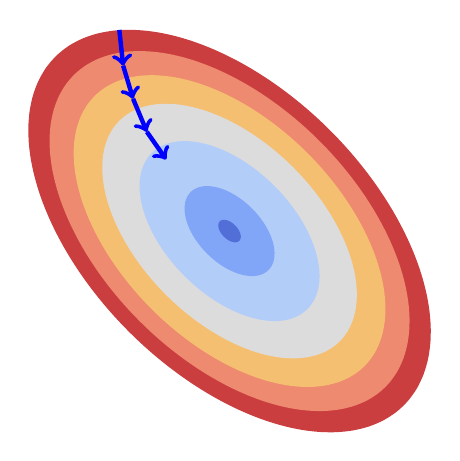
\begin{tikzpicture}[samples=100,smooth,scale=0.7]
			\begin{scope}
				\draw[opacity=0,fill=GDFirst,fill opacity=1] plot[domain=0:360] ({cos(\x)*sqrt(20/(sin(2*\x)+2))},{sin(\x)*sqrt(20/(sin(2*\x)+2))});
				\draw[opacity=0,fill=GDSecond,fill opacity=1] plot[domain=0:360] ({cos(\x)*sqrt(16/(sin(2*\x)+2))},{sin(\x)*sqrt(16/(sin(2*\x)+2))});
				\draw[opacity=0,fill=GDThird,fill opacity=1] plot[domain=0:360] ({cos(\x)*sqrt(12/(sin(2*\x)+2))},{sin(\x)*sqrt(12/(sin(2*\x)+2))});
				\draw[opacity=0,fill=GDFourth,fill opacity=1] plot[domain=0:360] ({cos(\x)*sqrt(8/(sin(2*\x)+2))},{sin(\x)*sqrt(8/(sin(2*\x)+2))});
				\draw[opacity=0,fill=GDFiveth,fill opacity=1] plot[domain=0:360] ({cos(\x)*sqrt(4/(sin(2*\x)+2))},{sin(\x)*sqrt(4/(sin(2*\x)+2))});
				\draw[opacity=0,fill=GDSixth,fill opacity=1] plot[domain=0:360] ({cos(\x)*sqrt(1/(sin(2*\x)+2))},{sin(\x)*sqrt(1/(sin(2*\x)+2))});
				\draw[opacity=0,fill=GDSeventh,fill opacity=1] plot[domain=0:360] ({cos(\x)*sqrt(0.0625/(sin(2*\x)+2))},{sin(\x)*sqrt(0.0625/(sin(2*\x)+2))});
			
				\draw[->,blue,ultra thick] (-2,3.65) to (-1.93,3);
				\draw[->,blue,ultra thick] (-1.93,3) to (-1.75,2.4);
				\draw[->,blue,ultra thick] (-1.75,2.4) to (-1.5,1.8);
				\draw[->,blue,ultra thick] (-1.5,1.8) to (-1.15,1.3);
			\end{scope}
		\end{tikzpicture}
  	\end{figure}
  	\end{minipage}
  \end{frame}
  \begin{frame}{ANN optimization \(\rightarrow\) Gradient Descent \& back-propagation}
  	The optimization is divided in two steps:
  	\begin{itemize}
  		\item{Compute of the gradient with back-propagation:
  			\begin{itemize}
  				\item{Forward phase}
  				\item{Backward phase and weights update}
  			\end{itemize}}
  	\end{itemize}
  	
  	We used \textbf{ADAM} (Adaptive Moment estimation) \cite{Kingma2014AdamAM} as gradient-based optimization algorithm:
  	\begin{itemize}
  		\item{Uses the concept of momentum to regularize the descent of the gradient}
  	\end{itemize}
  \end{frame}
  \begin{frame}{ANN optimization \(\rightarrow\) Alternatives}
  	\begin{itemize}
  		\item{Gradient Descent and back-propagation are powerful}
  		\item{Alternative is in Evolutionary Algorithm
  			\begin{itemize}
  				\item{Avoid the necessity of differentiable functions.}
  			\end{itemize}}
  	\end{itemize}
  \end{frame}
  \fi
  \section{Neural Network optimization \& DENN}
  \setbeamercolor{palette primary}{fg=mFG_DE, bg=mBG_DE}
  \begin{frame}{NN optimization \& DENN \(\rightarrow\) Gradient Descent \& back-propagation}
  	Gradient Descent and back-propagation optimization is divided in \textbf{computing of the gradient} and \textbf{updating of the network parameters}.\newline\newline
  	We used \textbf{ADAM} (Adaptive Moment estimation) \cite{Kingma2014AdamAM} as in \cite{NRAM:2016} as gradient-based optimization algorithm. Uses the concept of \textbf{momentum} to regularize the descent of the gradient.
  \end{frame}
  \begin{frame}{NN optimization \& DENN \(\rightarrow\) Differential Evolution}
  	Differential Evolution
  	\begin{itemize}  		
  		\item{Meta-heuristic}
  		\item{Searches a solution through the parallel evolution of a set of candidate solutions}
  		\item{Candidate solutions set called \textbf{population}
  			\begin{itemize}
  				\item{Composed by \textbf{N} D-dimensional numerical vectors, called \textbf{Individuals}}
  			\end{itemize}}
  	\end{itemize}
  \end{frame}
  \begin{frame}{NN optimization \& DENN \(\rightarrow\) Differential Evolution}
  	Its functioning is iterative
  	\vspace{-0.175cm}
  	\begin{enumerate}
  		\item{\textbf{Mutation}: driven by a constant $F$ creates a new population called \textbf{donor set} (several methods, e.g. \textbf{DEGL} and \textbf{Current-to-pbest})}
  		\item{\textbf{Crossover}: driven by a constant $CR$ creates a new population called \textbf{trial set} (several methods, e.g. \textbf{bin})}
  		\item{\textbf{Selection}: generates the new population for the next generation comparing one-by-one the trial vectors with the corresponding target vectors.}
  	\end{enumerate}
  	\vspace{-0.175cm}
  	Exist various self-adaptive variants of Differential Evolution which alleviate the problem dependence of $F$ and $CR$:
  	\vspace{-0.175cm}
  	\begin{itemize}
  		\item{\textbf{JADE}}
  		\item{\textbf{SHADE}}
  		\item{\textbf{L-SHADE}}
  	\end{itemize}
  \end{frame}
  \iffalse
  \begin{frame}{DE \& DENN \(\rightarrow\) Mutation}
  	Through the \textbf{mutation phase} a new population, called \textbf{donor set}, is created. Let $x$ an individual at the generation $G$, also called target. A donor is generated combining $x$ with some other individuals through a differential mutation operator. 
  \end{frame}
  \begin{frame}{DE \& DENN \(\rightarrow\) Mutation \(\rightarrow\) Variants}
  	Some variants used in the thesis are the following:
  	\begin{itemize}
  		\item{\textbf{DEGL}: generates a donor $u_i = w \cdot \textbf{G}_{i, G} + (1 - w) \cdot \textbf{L}_{i, G}$ where:
  			\begin{itemize}
  				\item{$w \in (0, 1)$}
  				\item{$\textbf{G}_{i, G} = \textbf{x}_{i, G} + \alpha \cdot (\textbf{x}_{\textit{g\_best}, G} - \textbf{x}_{i, G}) + \beta \cdot (\textbf{x}_{r_1, G} - \textbf{x}_{r_2, G})$}
  				\item{$\textbf{L}_{i, G} = \textbf{x}_{i, G} + \alpha \cdot (\textbf{x}_{\textit{n\_best}_i, G} - \textbf{x}_{i, G}) + \beta \cdot (\textbf{x}_{p, G} - \textbf{x}_{q, G})$}
			\end{itemize}}
  		\item{\textbf{Current-to-pbest}: \begin{center}$\textbf{u}_{i, G} = \textbf{x}_{i, G} + F_i \cdot (\textbf{x}_{\textrm{p\_best}, G} - \textbf{x}_{i, G}) + F_i \cdot (\textbf{x}_{r_1, G} - \textbf{x}_{r_2, G})$\end{center}where $x_{\textrm{p\_best}}$ is the individual selected in the 100p\% best individuals.}
	\end{itemize}
  \end{frame}
  \begin{frame}{DE \& DENN \(\rightarrow\) Crossover}
  	The \textbf{crossover phase} does nothing else than mixing up one-by-one the donor vectors components with the target vectors with some crossover methods, generating the \textbf{trials set} and enhancing the potential diversity of the population (a better exploration). 
  \end{frame}
  \begin{frame}{DE \& DENN \(\rightarrow\) Crossover \(\rightarrow\) Bin}
  	For example, let the target vector $x_{i,G}$ and the mutant $v_{i,G}$ the \textbf{bin} strategy work as follows
	\begin{center}
		$u_{ji, G} = \begin{cases}
			v_{ji,G}, & \textrm{if}\ (\textit{randb}(j) \leq \textit{CR})\ \textrm{or}\ j=\textit{rnbr}(i)\\
			x_{ji,G}, & otherwise
		\end{cases}$
	\end{center}
  \end{frame}
  \begin{frame}{DE \& DENN \(\rightarrow\) Crossover \(\rightarrow\) Bin \(\rightarrow\) Example}
	\begin{figure}
		\centering
		\includegraphics[width=0.8\textwidth]{../figures/bin-0.png}
	\end{figure}
  \end{frame}
  
  \begin{frame}{DE \& DENN \(\rightarrow\) Crossover \(\rightarrow\) Bin \(\rightarrow\) Example}
	\begin{figure}
		\centering
		\includegraphics[width=0.8\textwidth]{../figures/bin-1.png}
	\end{figure}
  \end{frame}
  
  \begin{frame}{DE \& DENN \(\rightarrow\) Crossover \(\rightarrow\) Bin \(\rightarrow\) Example}
	\begin{figure}
		\centering
		\includegraphics[width=0.8\textwidth]{../figures/bin-2.png}
	\end{figure}
  \end{frame}
  
  \begin{frame}{DE \& DENN \(\rightarrow\) Crossover \(\rightarrow\) Bin \(\rightarrow\) Example}
	\begin{figure}
		\centering
		\includegraphics[width=0.8\textwidth]{../figures/bin-3.png}
	\end{figure}
  \end{frame}
  
  \begin{frame}{DE \& DENN \(\rightarrow\) Crossover \(\rightarrow\) Bin \(\rightarrow\) Example}
	\begin{figure}
		\centering
		\includegraphics[width=0.8\textwidth]{../figures/bin-4.png}
	\end{figure}
  \end{frame}
  \begin{frame}{DE \& DENN \(\rightarrow\) Selection}
	Each trial is compared one-by-one to the corresponding target using the fitness function - if the target have a smaller cost with respect to the trial, than it is retained as individual of the population of the next generation and vice-versa.
  \end{frame}
  \begin{frame}{NN optimization \& DENN \(\rightarrow\) Differential Evolution \(\rightarrow\) Variants}
  	There exist various DE variants; we used:
  	\begin{itemize}
  		\item{\textbf{JADE}: generates at each generation $\textrm{F}_i$ and $\textrm{CR}_i$ for each target $x_i$, through $\mu_{\textrm{F}}$ and $\mu_{\textrm{CR}}$} 
  		\item{\textbf{SHADE}: generates $\textrm{F}_i$ and $\textrm{CR}_i$ for each target $x_i$, with an adaptation system based on two memories $M_{\textrm{F}}$ and $M_{\textrm{CR}}$ of \textit{finite} size $H$, called \textit{historical memories}, updated with $S_{\textrm{F}}$ and $S_{\textrm{CR}}$;}
  		\item{\textbf{L-SHADE}: similar to SHADE, but at every generation it reduces linearly the population.}
  	\end{itemize}
  \end{frame}
  \fi
  
  \begin{frame}{NN optimization \& DENN \(\rightarrow\) DENN (Differential Evolution for Neural Network)}
  	DENN \cite{denn2017mod} is a \textbf{framework} which implements the concepts of the Differential Evolution to train ANN:
  	\begin{itemize}
		\item{Created by Gabriele Di Bari and Mirco Tracolli}
		\item{It is written in C++ based on the library Eigen}
		\item{Each individual is composed by the weights and biases of the network}
		\item{The mutation and crossover operators are applied in a component-wise way}
	\end{itemize}
  \end{frame}
  \section{Implementation \& Faced problems}
  \setbeamercolor{palette primary}{fg=mFG_IMP, bg=mBG_IMP}
  \begin{frame}{Implementation \& Faced problems \(\rightarrow\) Description}
  \begin{minipage}{0.58\textwidth}
  	Three applications 
  	\begin{itemize}
  		\item{\textbf{NRAM-DENN}: training with Differential Evolution}
  		\item{\textbf{NRAM-Theano}: training with Gradient Descent-ADAM}
  		\item{\textbf{NRAM-Tester}: execution and generalization testing}
  	\end{itemize}
  \end{minipage}
  \hfill
  \begin{minipage}{0.4\textwidth}
  	\begin{figure}
  		\centering
  		\includegraphics[width=\textwidth]{../figures/nram-implementation.png}
  	\end{figure}
  \end{minipage}	
  \end{frame}
  \begin{frame}{Implementation \& Faced problems \(\rightarrow\) Additional used techniques}
  	\begin{itemize}
  		\item[]{\textbf{NRAM-Theano}:
  			\begin{itemize}
  				\item{\textbf{Gradient clipping}: gradient clipped in $[C_1,C_2]$ to avoid the common problem of the Gradient Explosion;}
  				\item{\textbf{Noise}: added a noise to the computed gradient to enhance the exploration;}
  			\end{itemize}
  		}
  		
  		\item[]{\textbf{NRAM-DENN}:
  			\begin{itemize}
  				\item{\textbf{Curriculum Learning}: it is used to enhance the training of the ANN through increasing difficulties of the datasets.}
  			\end{itemize}
  		}
  	\end{itemize}
  \end{frame}
\begin{frame}{Implementation \& Faced problems \(\rightarrow\) Problems}
  	Tested problems:
  	\begin{itemize}
  		\item{\textbf{Access}: accessing of a value of an input sequence}
  		\item{\textbf{Increment}: incrementing by one of a input sequence}
  		\item{\textbf{Copy}: copying an input sequence to a part of the memory}
  		\item{\textbf{Reverse}: copying an input sequence in a reverse order to a part of the memory}
  	\end{itemize}
  \end{frame}  
  
  \iffalse
  \begin{frame}{Implementation \& Faced problems \(\rightarrow\) Problems}
  	Tested problems:
  	\begin{itemize}
  		\item{\textbf{Access}: the access of a value of an input sequence
			\begin{table}
				\resizebox{0.725\textwidth}{!}{\begin{tabular}{|c|c|c|c|c|c|c|c|c||c|c|c|c|c|c|c|c|c|}					
					\hline
					\multicolumn{9}{|c||}{\textbf{Initial memory content}} & \multicolumn{9}{c|}{\textbf{Expected memory content}} \\ \hline
			\textbf{5} & 5 & 1 & 4 & 7 & \underline{4} & 1 & 2 & 0 & \textbf{4} & 5 & 1 & 4 & 7 & \underline{4} & 1 & 2 & 0 \\ \hline
				\end{tabular}}
			\end{table}  		
  		}
  		\item{\textbf{Increment}: the increment by one of a input sequence
			\begin{table}
				\resizebox{0.725\textwidth}{!}{\begin{tabular}{|c|c|c|c|c|c|c|c|c||c|c|c|c|c|c|c|c|c|}					
					\hline
					\multicolumn{9}{|c||}{\textbf{Initial memory content}} & \multicolumn{9}{c|}{\textbf{Expected memory content}} \\ \hline
			5 & 6 & 4 & 2 & 7 & 1 & 4 & 2 & 0 & 6 & 7 & 5 & 3 & 8 & 2 & 5 & 3 & 0 \\ \hline
				\end{tabular}}
			\end{table}}
  		\item{\textbf{Copy}: the copy in another part of the memory of an input sequence
  		\begin{table}
				\resizebox{0.725\textwidth}{!}{\begin{tabular}{|c|c|c|c|c|c|c|c|c||c|c|c|c|c|c|c|c|c|}					
					\hline
					\multicolumn{9}{|c||}{\textbf{Initial memory content}} & \multicolumn{9}{c|}{\textbf{Expected memory content}} \\ \hline
			\textbf{5} & 6 & 4 & 2 & 7 & \underline{0} & 0 & 0 & 0 & 5 & 6 & 4 & 2 & 7 & \textbf{6} & \textbf{4} & \textbf{2} & \textbf{7} \\ \hline
				\end{tabular}}
			\end{table}}
  		\item{\textbf{Reverse}: the reversed copy in another part of the memory of an input sequence
  		\begin{table}
				\resizebox{0.725\textwidth}{!}{\begin{tabular}{|c|c|c|c|c|c|c|c|c||c|c|c|c|c|c|c|c|c|}					
					\hline
					\multicolumn{9}{|c||}{\textbf{Initial memory content}} & \multicolumn{9}{c|}{\textbf{Expected memory content}} \\ \hline
			\textbf{5} & 6 & 4 & 2 & 7 & \underline{0} & 0 & 0 & 0 & 5 & 6 & 4 & 2 & 7 & \textbf{7} & \textbf{2} & \textbf{4} & \textbf{6} \\ \hline
				\end{tabular}}
		\end{table}}
  	\end{itemize}
  \end{frame}
  \begin{frame}{Implementation \& Faced problems \(\rightarrow\) Problems \(\rightarrow\) Access}
	Given a value $k$ and an array \textbf{A}, return $\textbf{A}[k]$. Input is given as $k, A[0], \dots, \textbf{A}[n-1], \textit{NULL}$ and the network should replace the first memory cell with $\textbf{A}[k]$. 
	\begin{table}[h!]
		\centering
		\resizebox{0.5\textwidth}{!}{\begin{tabular}{|c|c|c|c|c|c|c|c|c|c|}
			\hline
			\multicolumn{10}{|c|}{\textbf{Initial memory}} \\ \hline
			\textbf{4} & 5 & 1 & 4 & \underline{7} & 2 & 8 & 3 & 6 & 0 \\ \hline\hline\hline
			\multicolumn{10}{|c|}{\textbf{Desired memory}} \\ \hline
			\textbf{7} & 5 & 1 & 4 & 7 & 2 & 8 & 3 & 6 & 0 \\ \hline\hline\hline
			\multicolumn{10}{|c|}{\textbf{Cost mask}} \\ \hline
			1 & 1 & 1 & 1 & 1 & 1 & 1 & 1 & 1 & 1 \\ \hline\hline\hline
			\multicolumn{10}{|c|}{\textbf{Error mask}} \\ \hline
			1 & 0 & 0 & 0 & 0 & 0 & 0 & 0 & 0 & 0 \\ \hline
		\end{tabular}}
	\end{table}
  \end{frame}
  \begin{frame}{Implementation \& Faced problems \(\rightarrow\) Problems \(\rightarrow\) Reverse}
  	Given an array and a pointer to the destination, copy all elements from the array in reversed order. Input is given as $p, \textbf{A}[0], \dots, \textbf{A}[n-1]$ where $p$ points one element after $\textbf{A}[n-1]$. The expected output is $\textbf{A}[n-1], \dots, \textbf{A}[0]$ at positions $p, \dots, p+n-1$.
  	\begin{table}[h!]
		\centering
		\resizebox{0.5\textwidth}{!}{\begin{tabular}{|c|c|c|c|c|c|c|c|c|}
			\hline
			\multicolumn{9}{|c|}{\textbf{Initial memory}} \\ \hline
			\textbf{5} & 5 & 1 & 4 & 7 & \underline{0} & 0 & 0 & 0 \\ \hline\hline\hline
			\multicolumn{9}{|c|}{\textbf{Desired memory}} \\ \hline
			\textbf{5} & 5 & 1 & 4 & 7 & 7 & 4 & 1 & 5 \\ \hline\hline\hline
			\multicolumn{9}{|c|}{\textbf{Cost mask}} \\ \hline
			0 & 1 & 1 & 1 & 1 & 1 & 1 & 1 & 1\\ \hline\hline\hline
			\multicolumn{9}{|c|}{\textbf{Error mask}} \\ \hline
			0 & 0 & 0 & 0 & 0 & 1 & 1 & 1 & 1 \\ \hline
	\end{tabular}}
	\end{table}
  \end{frame}
  \fi
  \begin{frame}{Implementation \& Faced problems \(\rightarrow\) Datasets}
  	\begin{minipage}{0.41\textwidth}
  		The datasets are generated at runtime; each batch of samples is composed by:
		\begin{itemize}
			\item{\textbf{initial memory content}}
			\item{\textbf{expected memory content}}
			\item{\textbf{cost mask}}
			\item{\textbf{error rate mask}}
		\end{itemize}
  	\end{minipage}
  	\hfill
  	\begin{minipage}{0.58\textwidth}
  		\begin{table}[h]
		\centering
		\resizebox{0.8\textwidth}{!}{\begin{tabular}{|c|c|c|c|c|c|c|c|c|}
			\hline
			\multicolumn{9}{|c|}{\textbf{Initial memory content}} \\ \hline
			\textbf{5} & 5 & 1 & 4 & 7 & \underline{0} & 0 & 0 & 0 \\ \hline\hline\hline
			\multicolumn{9}{|c|}{\textbf{Expected memory content}} \\ \hline
			\textbf{5} & 5 & 1 & 4 & 7 & 7 & 4 & 1 & 5 \\ \hline\hline\hline
			\multicolumn{9}{|c|}{\textbf{Cost mask}} \\ \hline
			0 & 1 & 1 & 1 & 1 & 1 & 1 & 1 & 1\\ \hline\hline\hline
			\multicolumn{9}{|c|}{\textbf{Error mask}} \\ \hline
			0 & 0 & 0 & 0 & 0 & 1 & 1 & 1 & 1 \\ \hline
			\end{tabular}}
			\caption{Reverse task.}
		\end{table}
  	\end{minipage}
  \end{frame}
  \iffalse
  \begin{frame}{Generalization}
  	Generalization means is the ability of a neural network to recognize patterns in new examples which were never seen before. Remembering how the training is made, here \textit{generalization} means the ability of the controller to generate the ``right'' circuits also with different parameters of the NRAM.
  \end{frame}
  \fi
  \section{Results, Conclusions \& Future works}
	\setbeamercolor{palette primary}{fg=mFG_RES, bg=mBG_RES}
  \begin{frame}{Results, Conclusions \& Future works \(\rightarrow\) Results \(\rightarrow\) DE \& GD results}
  
  	\begin{table}[t]
	\centering

	\rowcolors{2}{mLightLightGray}{mLightGray}
		\resizebox{0.9\textwidth}{!}{
			\begin{tabular}{ccccccccc}
				\rowcolor{Gray} \textbf{Task} & \multicolumn{2}{c}{\textbf{Train complexity}} & \multicolumn{2}{c}{\textbf{Reached cost 0}} & \multicolumn{2}{c}{\textbf{Train error}} & \multicolumn{2}{c}{\textbf{Generalization}} \\
				\rowcolor{Gray} & No CL & CL & No CL & CL & No CL & CL & No CL & CL \\ \hline
		
				Access & --- & $\textrm{len}(A) \leq 20$ & $\times$  & \checkmark & --- & 0 & $\times$  & Perfect \\ 
				Increment & 	--- & $\textrm{len}(A) \leq 15$  & $\times$ & \checkmark & --- & 0 & $\times$  & Perfect \\
				Copy & --- & $\textrm{len}(A) \leq 15$ & $\times$ & \checkmark & --- & 0 & $\times$ & Perfect \\ 
				Reverse & --- & $\textrm{len}(A) \leq 15$ & $\times$  & \checkmark & --- & 0 & $\times$  & Perfect \\ 
			\end{tabular}
		}
		\caption{Results of the tests with ADAM in \cite{NRAM:2016}.}
	\end{table}
	\vspace{-0.5cm}
  	\begin{table}[t]
	\centering

	\rowcolors{2}{mLightLightGray}{mLightGray}
		\resizebox{0.9\textwidth}{!}{
			\begin{tabular}{ccccccccc}
				\rowcolor{Gray} \textbf{Task} & \multicolumn{2}{c}{\textbf{Train complexity}} & \multicolumn{2}{c}{\textbf{Reached cost 0}} & \multicolumn{2}{c}{\textbf{Train error}} & \multicolumn{2}{c}{\textbf{Generalization}} \\
				\rowcolor{Gray} & No CL & CL & No CL & CL & No CL & CL & No CL & CL \\ \hline
		
				Access & \begin{tabular}{@{}c}$\textrm{len}(A) = 8$ \\ $t = 5$\end{tabular} & $\textrm{len}(A) \leq 10$ & \checkmark & \checkmark & 0 & 0 & Perfect & Perfect \\ 
				Increment & 	\begin{tabular}{@{}c}$\textrm{len}(A) = 9$\\$t = 4$\end{tabular}& $\textrm{len}(A) \leq 10$  & \checkmark & \checkmark & 0 & 0 & Perfect & Perfect \\
				Copy & 	\begin{tabular}{@{}c}$\textrm{len}(A) = 5$\\$t = 11$\end{tabular} & $\textrm{len}(A) \leq 9$  & $\times$ & $\times$ & --- & --- & --- & --- \\ 
				Reverse & \begin{tabular}{@{}c}$\textrm{len}(A) = 4$\\$t = 9$\end{tabular} & $\textrm{len}(A) \leq 8$ & \checkmark & \checkmark & 0 & 0 & Perfect & Perfect \\ 
			\end{tabular}
		}
		\caption{Results of the tests with Differential Evolution.}
	\end{table}
	
	
  \end{frame}
  \if 0
	\begin{table}[t]
		\centering
	
		\rowcolors{2}{mLightGray}{mLightLightGray}
		\resizebox{0.6\textwidth}{!}{\begin{tabular}{ccc}
		\rowcolor{Gray} \textbf{Task} & \textbf{Train complexity} & \textbf{Reached cost 0} \\ \hline
		Access & $\textrm{len}(A) = 8, t = 5$ & $\times$ \\ 
		Increment & $\textrm{len}(A) = 9, t = 4$ & $\times$ \\
		Copy & $\textrm{len}(A) = 5, t = 11$  & $\times$  \\ 
		Reverse & $\textrm{len}(A) = 4, t = 9$  & $\times$ \\ 
		\end{tabular}}
		\caption{Results of the tests with back-propagation and ADAM.}
	\end{table}
	\fi
  \begin{frame}{Results, Conclusions \& Future works \(\rightarrow\) Results \(\rightarrow\) DE \& GD results}
  	\begin{table}[t]
	\centering
	\rowcolors{2}{mLightLightGray}{mLightGray}
	\resizebox{\linewidth}{!}{\begin{tabular}{l|cccccccccccc}
	\rowcolor{Gray} \textbf{Task} & \multicolumn{2}{c}{\textbf{JADE/DEGL/1}} & \multicolumn{2}{c}{\textbf{JADE/c-to-pb/1}} & \multicolumn{2}{c}{\textbf{SHADE/DEGL/1}} & \multicolumn{2}{c}{\textbf{SHADE/c-to-pb/1}}\\
		\rowcolor{Gray} & No CL & CL & No CL & CL & No CL & CL & No CL & CL \\ \hline
		Access & $\times$ & \checkmark & \checkmark & \checkmark & $\times$ & $\times$ & $\times$ & \checkmark  \\
		Increment & $\times$ & $\times$ & \checkmark & $\times$ & $\times$ & $\times$ & $\times$ & \checkmark \\
		Copy & $\times$ & $\times$ & $\times$ & $\times$ & $\times$ & $\times$ & $\times$ & $\times$ \\
		Reverse & $\times$ & \checkmark & \checkmark & $\times$ & \checkmark & \checkmark & $\times$ & \checkmark \\
	\end{tabular}}
	\caption{Results of DE variants}
\end{table}
  \end{frame}
  \begin{frame}{Results, Conclusions \& Future works \(\rightarrow\) Charts of convergence \(\rightarrow\) Access}
	\begin{figure}[h]
		\centering
		\resizebox{\textwidth}{!}{\begin{tikzpicture}[smooth]
			\begin{axis}[  				
  				xlabel={$\textrm{Generation}$},
  				ylabel={$\textrm{Cost}$},
  				xlabel style={below right},
  				ylabel style={above left},	
			    xmin=0, xmax=350,
				legend pos=outer north east,
				cycle list name=colors tesi
			]
  				\addplot +[mark=none] table{../data/access/adam};
  				\addlegendentry{ADAM}

  				\addplot +[mark=none] table{../data/access/jade_degl};
  				\addlegendentry{JADE/DEGL/1/bin}

  				\addplot +[mark=none] table{../data/access/jade_degl_cl};
  				\addlegendentry{JADE/DEGL/1/bin + CL}
  				
  				\addplot +[mark=none] table{../data/access/jade_curr_p_best};
  				\addlegendentry{JADE/Current-to-pbest/1/bin}
  				
  				\addplot +[mark=none] table{../data/access/jade_curr_p_best_cl};
  				\addlegendentry{JADE/Current-to-pbest/1/bin + CL}

  				\addplot +[mark=none] table{../data/access/shade_degl};
  				\addlegendentry{SHADE/DEGL/1/bin}

  				\addplot +[mark=none] table{../data/access/shade_degl_cl};
  				\addlegendentry{SHADE/DEGL/1/bin + CL}
  				
  				\addplot +[mark=none] table{../data/access/shade_curr_p_best};
  				\addlegendentry{SHADE/Current-to-pbest/1/bin}
  				
  				\addplot +[mark=none] table{../data/access/shade_curr_p_best_cl};
  				\addlegendentry{SHADE/Current-to-pbest/1/bin + CL}

			\end{axis}
		\end{tikzpicture}}
	\end{figure}
  \end{frame}
  \begin{frame}{Results, Conclusions \& Future works \(\rightarrow\) Charts of convergence \(\rightarrow\) Reverse}
  	\begin{figure}[h]
		\centering
		\resizebox{\textwidth}{!}{\begin{tikzpicture}[smooth]
			\begin{axis}[  				
  				xlabel={$\textrm{Generation}$},
  				ylabel={$\textrm{Cost}$},
  				xlabel style={below right},
  				ylabel style={above left},	
			    xmin=0, xmax=1000,
				legend pos=outer north east,
				cycle list name=colors tesi
			]
  				\addplot +[mark=none] table{../data/reverse/adam.txt};
  				\addlegendentry{ADAM}

  				\addplot +[mark=none] table{../data/reverse/jade_degl.txt};
  				\addlegendentry{JADE/DEGL/1/bin}

  				\addplot +[mark=none] table{../data/reverse/jade_degl_cl.txt};
  				\addlegendentry{JADE/DEGL/1/bin + CL}
  				
  				\addplot +[mark=none] table{../data/reverse/jade_curr_p_best.txt};
  				\addlegendentry{JADE/Current-to-pbest/1/bin}
  				
  				\addplot +[mark=none] table{../data/reverse/jade_curr_p_best_cl.txt};
  				\addlegendentry{JADE/Current-to-pbest/1/bin + CL}

  				\addplot +[mark=none] table{../data/reverse/shade_degl.txt};
  				\addlegendentry{SHADE/DEGL/1/bin}

  				\addplot +[mark=none] table{../data/reverse/shade_degl_cl.txt};
  				\addlegendentry{SHADE/DEGL/1/bin + CL}
  				
  				\addplot +[mark=none] table{../data/reverse/shade_curr_p_best.txt};
  				\addlegendentry{SHADE/Current-to-pbest/1/bin}
  				
  				\addplot +[mark=none] table{../data/reverse/shade_curr_p_best_cl.txt};
  				\addlegendentry{SHADE/Current-to-pbest/1/bin + CL}

			\end{axis}
		\end{tikzpicture}}
		\label{fig:reverse-costs}
	\end{figure}
  \end{frame}
  \begin{frame}{Results, Conclusions \& Future works \(\rightarrow\) Circuits \(\rightarrow\) Access}
  	\begin{figure}
  		\centering
  		\includegraphics[width=\textwidth]{../figures/access-circuits.png}
  	\end{figure}
  \end{frame}
  \begin{frame}{Results, Conclusions \& Future works \(\rightarrow\) Circuits \(\rightarrow\) Reverse}
  	\begin{figure}
  		\centering
  		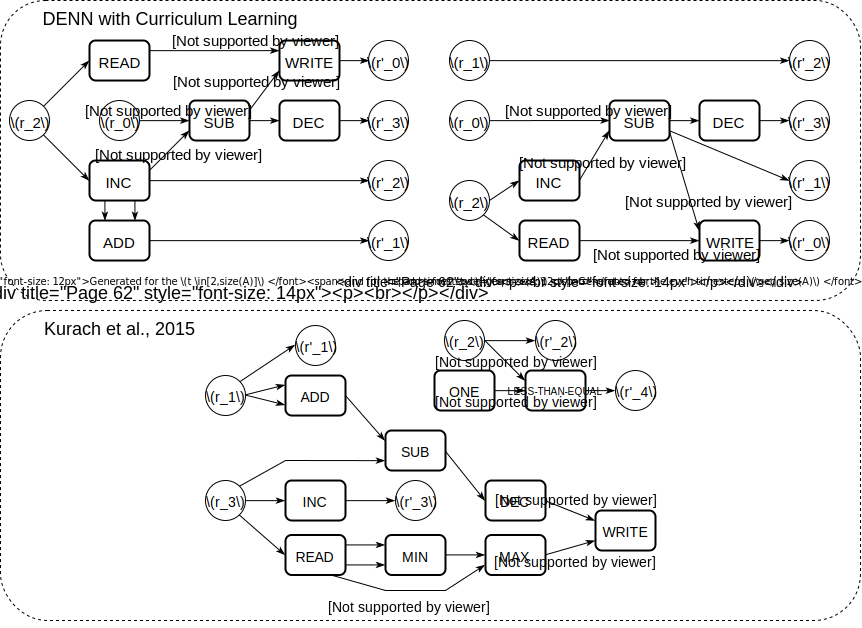
\includegraphics[width=\textwidth]{../figures/reverse-circuits.png}
  	\end{figure}
  \end{frame}
  \begin{frame}{Results, Conclusions \& Future works \(\rightarrow\) Conclusions}
  	DENN behave well in this type of model:
	\begin{itemize}
		\item{Differential Evolution behave differently with these problems w.r.t. ADAM producing different results}
		\item{Best performing variants are those with \textbf{Current-to-pbest}}
		\item{Found controllers generate simpler circuits w.r.t. in \cite{NRAM:2016}}
	\end{itemize}
  \end{frame}
  \begin{frame}{Results, Conclusions \& Future works \(\rightarrow\) Future works}
  	Create a new dynamic system for the gate selection.
  
	Write an enhanced NRAM model that does not require the differentiability condition.
  \end{frame}
  
  \setbeamercolor{palette primary}{fg=mFG_STAND, bg=mBG_STAND}
  \begin{frame}[standout]
  	Thanks for the attention!
  	\thispagestyle{empty}
  \end{frame}
  \begin{frame}<0>[noframenumbering]{References}
        \bibliography{bibliography}
  \end{frame}
\end{document}